\documentclass[a4paper]{scrartcl}
\usepackage[T1]{fontenc}
\usepackage[latin9]{inputenc}
\usepackage[ngerman]{babel}
\usepackage{graphicx}
\usepackage{amsmath}
\usepackage{color}
\usepackage{float}
\usepackage{longtable}
\usepackage{multirow}
\usepackage{rotating}
\usepackage{rotfloat}
\begin{document}
\titlehead{Professionelle Audioentwicklung - SS 2013}
\title{Software Design Document}
\publishers{HAW - Hochschule f�r Angewandte Wissenschaften Hamburg}
\maketitle

\vfill

\begin{tabular}{|r|l|}
\hline
Version & 0.8\\
\hline
Datum & 10.06.2013\\
\hline
Dokumenten Status & In Arbeit\\
\hline
\end{tabular}

\pagebreak

\textbf{�nderungshistory}

\vspace{\baselineskip}

\begin{tabular}{|l|l|l|l|}
\hline
\textbf{Version} & \textbf{Datum} & \textbf{Autor} & \textbf{�nderungen}\\
\hline
0.7 & 01.06.2013 & J. Meih�fer & Entwurf\\
\hline
0.8 & 10.06.2013 & J.Meih�fer & Architektur \& Java Server\\
\hline
\end{tabular}

\pagebreak

\tableofcontents

\pagebreak

\section{Ziel}

\subsection{Einleitung}
Dieses Software Design Dokument beschreibt das Softwaredesign f�r eine interaktive Audioinstallation. Dabei f�hrt ein virtuelles Auto je nach Geschwindigkeit eines Modellfahrzeugs mehr oder weniger schnell von einem Ort zum n�chsten. Je nach Ort wird eine Schallquelle auf einer Wellenfeldsynthese - Anlage ausgegeben. \\

\subsection{Systembeschreibung}


\begin{figure}[H]
\center
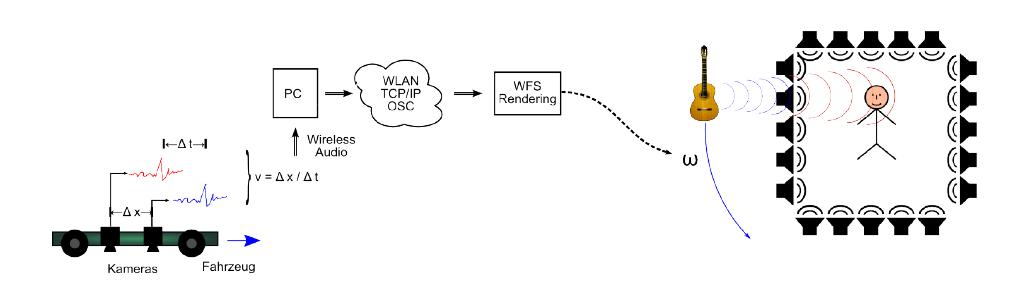
\includegraphics[width=15cm]{interakt_wfs}
\caption{Abbildung des Systems}
\end{figure}

Ein Modellfahrzeug f�hrt �ber einen strukturierten Boden, so dass �ber einen optischen Sensor unterschiede beim fahren zu erkennen sind. Durch den Abgleich zweier optischer Sensoren die unter dem Auto mit geringen Abstand hinter einander befestigt sind kann die Geschwindigkeit des Autos ermittelt werden. Dies geschieht indem ein PC die Daten des Modellfahrzeugs erh�lt, die Daten auswertet und so eine Geschwindigkeit ermittelt. Mittels OSC - Nachricht wird die ermittelte Geschwindigkeit an einen weiteren PC weitergeleitet. Dieser wertet dann die Geschwindigskeitsdaten aus und stuert mittels OSC die Soundquellen in Cubase an, sowie die Positionsangabe im Raum bei SWonder. Cubase wird wiederrum mit einer virtuellen Soundkarte verbunden �ber die dann die Soundquellen auf der Wellenfeld-Synthese-Anlage ausgegeben werden.\\

\subsection{Referenzmaterial}

\begin{tabular}{|c|c|c|}
\hline
\textbf{Dokument} & \textbf{Name} & \textbf{Version}\\
\hline
Liblo Funktionen & http://liblo.sourceforge.net/docs/modules.html & 0.27 \\
\hline
\end{tabular}

\subsection{Abk�rzungen}

\begin{tabular}{|l|l|}
\hline
Abk�rzung & Bedeutung\\
\hline
OSC & Open Sound Control\\
\hline
PC & Personal Computer\\
\hline
\end{tabular}

\section{Architektur}

\begin{figure}[H]
\center
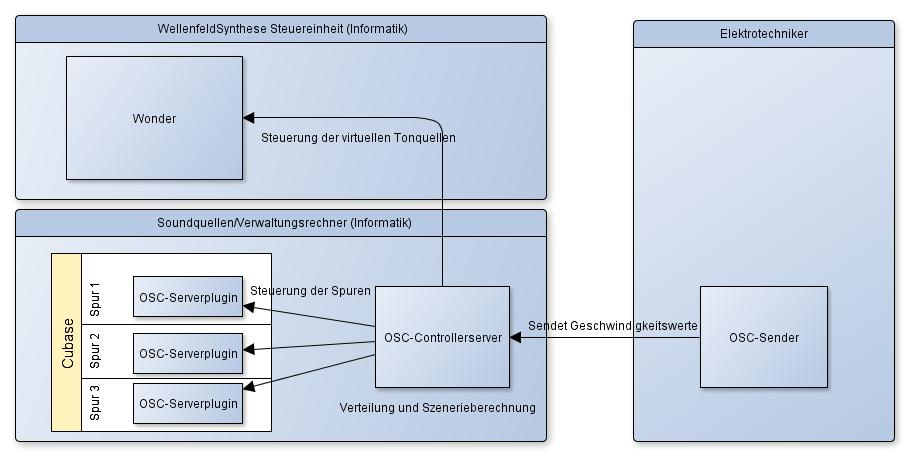
\includegraphics[width=15cm]{Architektur}
\end{figure}

Der OSC-Sender bekommt die Daten des Modellfahrzeugs �bergeben. Hier werden diese dann ausgewertet und mittels eines OSC-Clients an den OSC-Controllerserver weitergeleitet. Der OSC-Controllerserver nimmt die Daten entgegen, passt die Geschwindigkeit des virtuellen Autos an und berechnet anhand davon wo sich das virtuelle Auto gerade befindet. In einem Cubase Projekt laufen mehrere Audiospuren die jeweils einen Ort representieren in einer Endlosschleife. Jeder dieser Audiospuren ist ein OSC-Serverplugin zugeordnet, welche per OSC - Server OSC - Nachrichten vom OSC-Controllerserver entgegennehmen und anhand dieser die Lautst�rke der Audiospuren regeln. Zus�tzlich wandert je nach Geschwindigkeit die Soundquelle mittels Wonder durch den Raum. Die Kommunikation findet auch hier mittels OSC - Nachrichten statt.\\

\subsection{Software Architektur}

\subsubsection{OSC - Controllerserver}
Der OSC Controllerserver bietet eine eigene GUI um neue Pfade(OSC und Wonder), f�r die Ansteuerung der Plugins in Cubase und der Quellen in Wonder, zu generieren.
Hierbei sind IP Adresse, f�r den Host der Plugins, sowie f�r den Rechner der Wonder Quellen, und die Ports f�r die OSC Nachrichten frei einstellbar.\\
Generiert der Nutzer neue Pfade so werden diese in einer Liste gespeichert, bei Bedarf kann diese Liste, �ber die GUI, auch in eine externe Datei gespeichert werden, sodass sie immer wieder abgerufen und geladen werden kann.\\
Starter der User nun die Anwendung so werden alle Pfade und somit auch die Plugins und Wonder Quellen initialisiert, da diese mittels OSC an die Pfade gebunden sind. Nach der Initialisierung pr�ft das Programm periodisch, ob neue Geschwindigkeitsdaten vorliegen (per OSC ankommend) und aktualisiert dann die Geschwindigkeit innerhalb des Programms. 
Zus�tzlich wird die zur�ckgelegte Strecke berechnet ($s = v*t$). Aus den gespeicherten Location Daten der Pfade und deren Offset kann dann bestimmt werden, wann eine Quelle (Cubase Plugin) ein oder ausgeblendet werden soll. Au�erdem werden gleichzeitig und nach dem selben Prinzip die Wonder Quellen bewegt.\\
Hierbei muss jedoch die Geschwindkeit und die Strecke an den zur verf�gungstehenden Raum der Wellenfeldsynthese angeglichen werden.\\
Zur besseren Veranschaulichung k�nnen die Algorithmen als Flussdiagramm unter \textbf{wichtige Algorithmen} angeschaut werden.\\

\subsubsection{Klassendiagramm OSC - Controllerserver}
Klassendiagramm f�r Java OSC - Controller Server, ohne Illposed OSC library.\\
\begin{sidewaysfigure}[H]
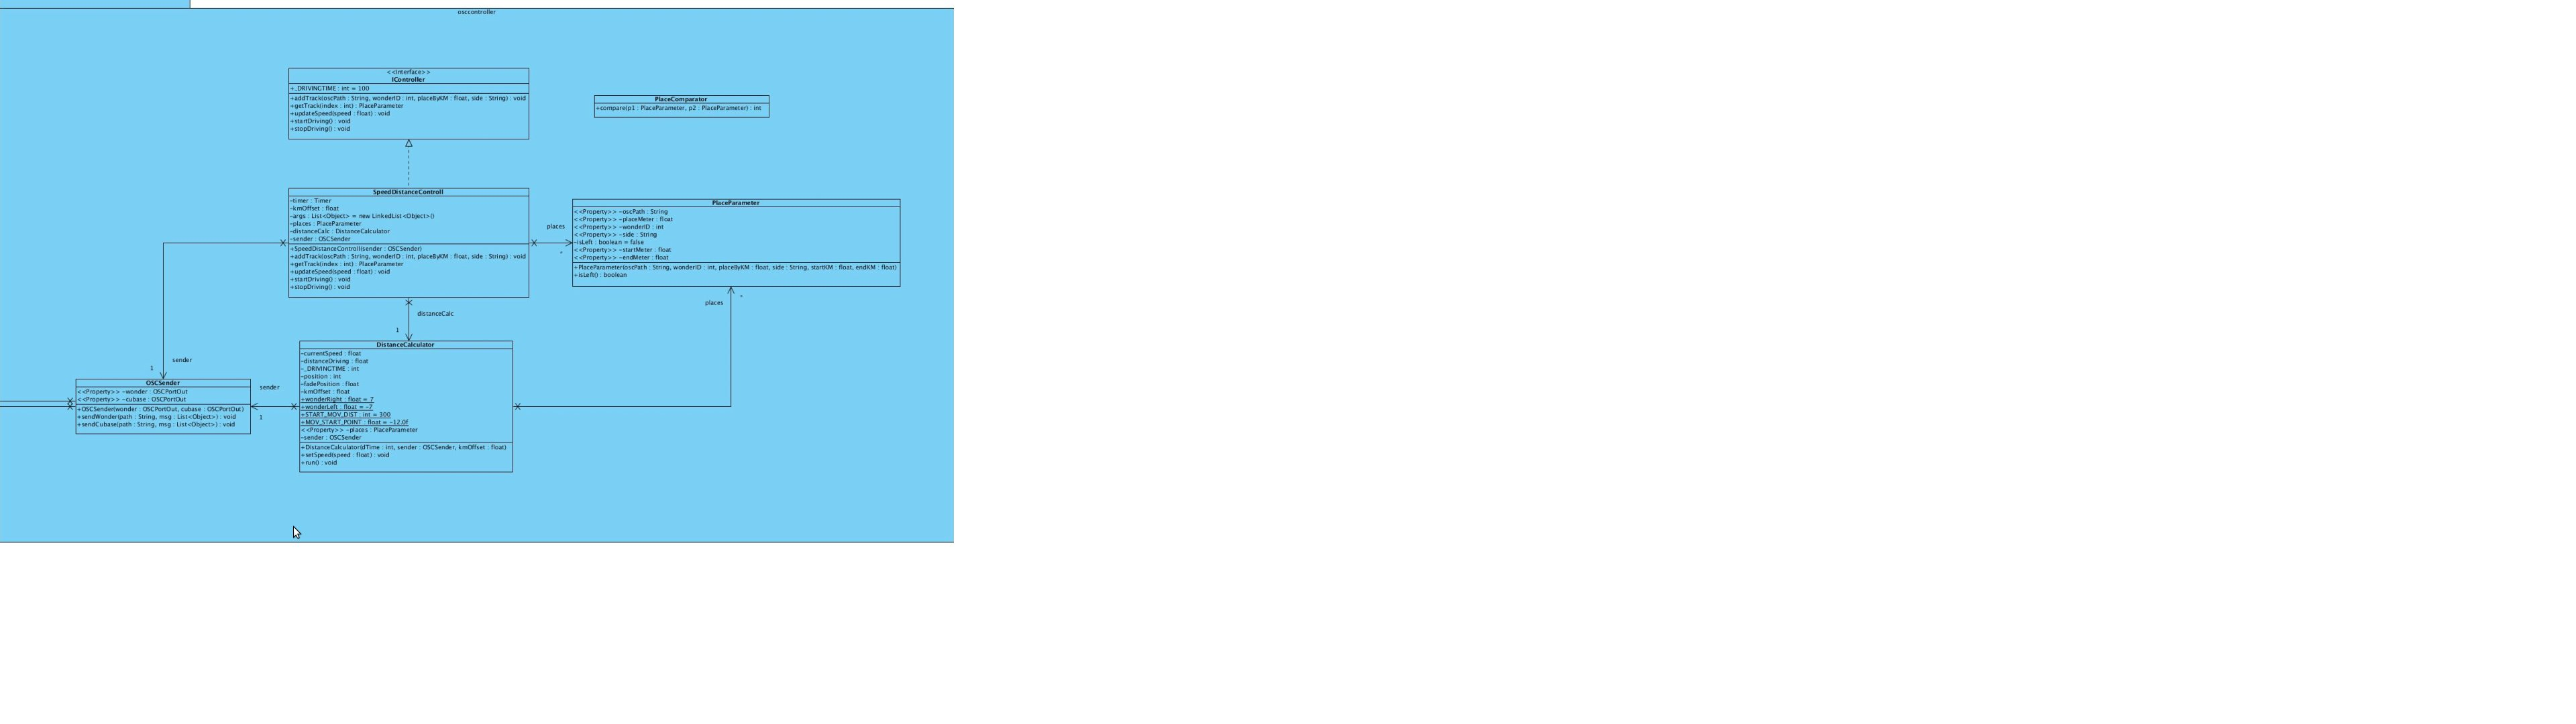
\includegraphics[width=20cm]{Klassendiagramm}
\end{sidewaysfigure}

\section{OSC}

\section{Interfaces}
\pagebreak
\section{Relevante Algorithmen}
\subsection{Java - OSC Controllerserver}
\begin{enumerate}
\item wird der Startbutton gedr�ckt, so werden die Quellen Initialisiert und auf einen definierten Startzustand gebracht.\\
\begin{figure}[H]
\center
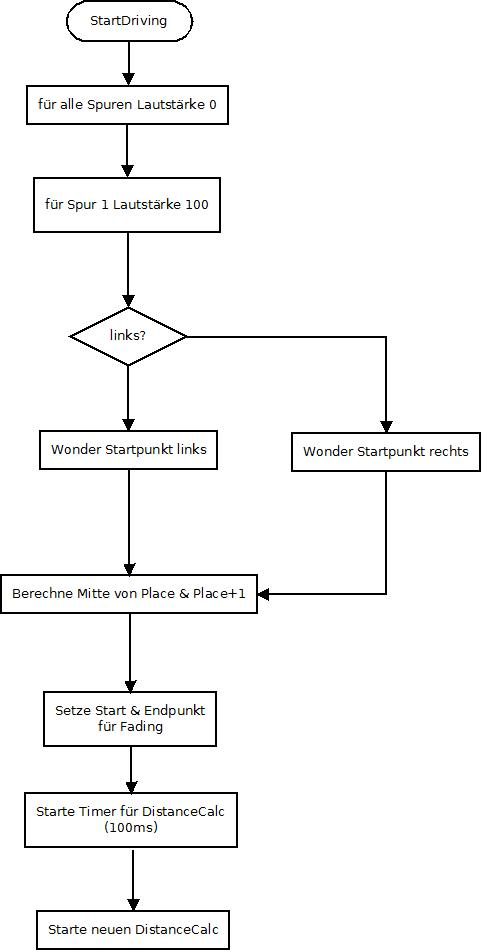
\includegraphics[width=8cm]{StartDriving}
\end{figure}
\pagebreak
\item Am Ende der Initialisierung wird der DistanceCalculator gestartet, sowie ein Timer f�r diesen initialisiert (100ms). Der DistanceCalculator wird alle 100ms aktiviert.\\
\begin{figure}[H]
\center
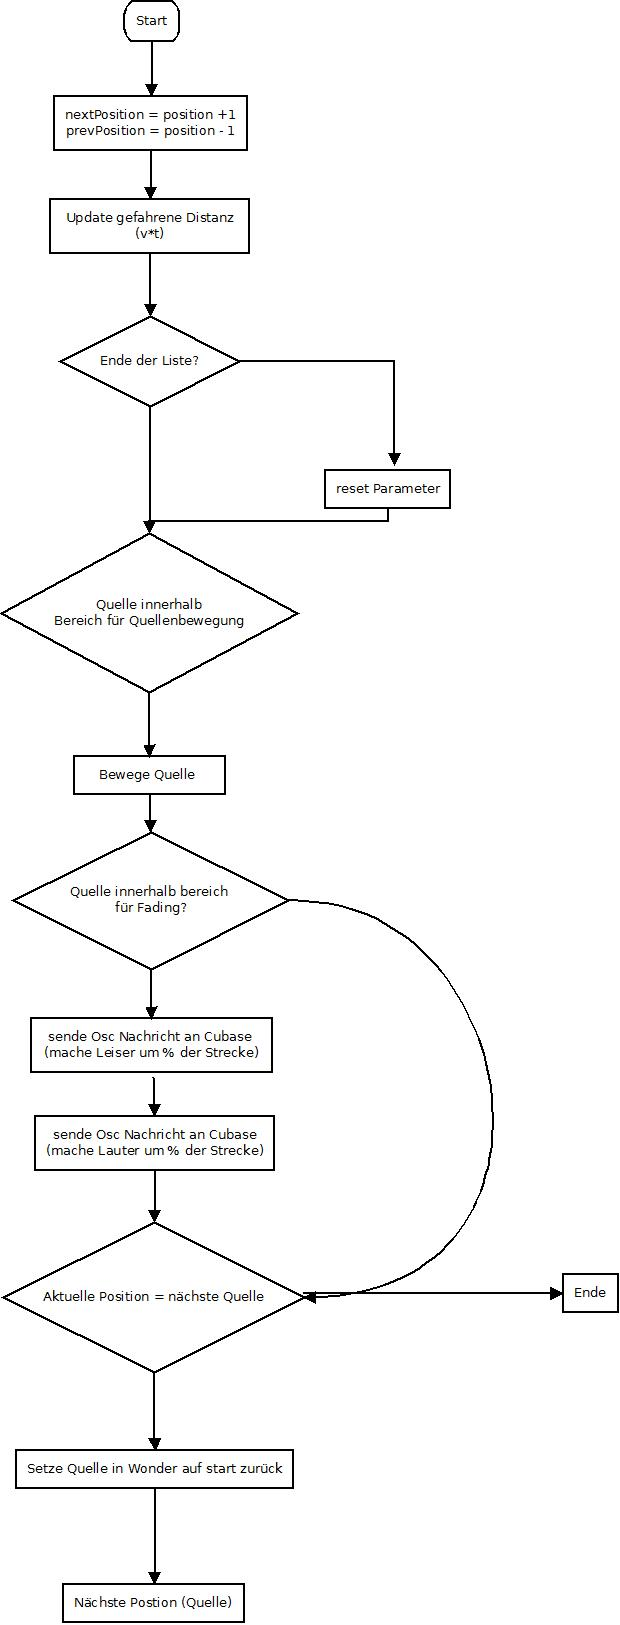
\includegraphics[width=7cm]{DistanceCalc}
\end{figure}
\end{enumerate}

\section{Parameter}

\subsection{OSC - Sender}

\begin{tabular}{|l|l|l|p{6cm}|}
\hline
\textbf{Lfd} & \textbf{Parameter} & \textbf{Werte} & \textbf{Beschreibung}\\
\hline
1 & ServerIP & IPv4-Adresse & IP - Adresse des PC's auf dem der OSC Controllerserver l�uft\\
\hline
2 & Port & int & Port f�r OSC Nachrichten im OSC Controllerserver\\
\hline
\end{tabular}

\subsection{OSC - Serverplugin}

\begin{tabular}{|l|l|l|p{6cm}|}
\hline
\textbf{Lfd} & \textbf{Parameter} & \textbf{Werte} & \textbf{Beschreibung}\\
\hline
1 & OSC Pfad & String & OSC Pfad auf den ein Plugin horcht\\
\hline
2 & Port & int & Port f�r OSC Nachrichten im Cubase Plugin\\
\hline
\end{tabular}

\subsection{OSC - Controllerserver}

\begin{tabular}{|l|l|l|p{6cm}|}
\hline
\textbf{Lfd} & \textbf{Parameter} & \textbf{Werte} & \textbf{Beschreibung}\\
\hline
1 & Cubase IP & localhost / IP - Adresse & IP - Adresse des PC's auf welchem Cubase l�uft.\\
\hline
2 & Cubase Port & int & Port auf welchem die Cubase - Plugins horchen.\\
\hline
3 & Wonder IP & localhost / IP - Adresse & IP - Adresse des PC's auf welchem Wonder l�uft.\\
\hline
4 & Wonder Port & int & Port auf welchem Wonder horcht.\\
\hline
5 & Local Path & /<Pfad> & OSC - Pfad auf welchem der OSC-Controllerserver OSC-Nachrichten entgegen nimmt.\\
\hline
6 & Local Port & int & Port auf welchem der OSC - Controllerserver horcht.\\
\hline
7 & OSC Path & /<Pfad> & OSC - Pfad auf welchem ein OSC - Serverplugin einer Audiospur OSC - Nachrichten entgegen nimmt.\\
\hline
8 & Wonder Src - ID & int >= 0 & ID der Soundquelle in Wonder.\\
\hline
9 & Position (KM) & float >= 0& Entfernung des virtuellen Ortes der Soundquelle in Kilometer.\\
\hline
10 & Passing Side & left / right & Seite auf welcher sich die Soundquelle in Wonder befindet.\\
\hline

\hline
\end{tabular}


\pagebreak

\section{Glossar}

\begin{tabular}{|c|c|}
\hline
\textbf{Begriff} & \textbf{Erl�uterung} \\
\hline
\hline
\end{tabular}

\end{document}
